
%(BEGIN_QUESTION)
% Copyright 2006, Tony R. Kuphaldt, released under the Creative Commons Attribution License (v 1.0)
% This means you may do almost anything with this work of mine, so long as you give me proper credit

Et biodieselanlegg i liten skala registrerer produksjonen av biodieseldrivstoff ved å måle væskenivå i et lagringskar. Det finnes ingen strømningstransmitter som måler strømningsraten inn i karet, men vi kan utlede strømningsraten ved å følge nivået over tid.

$$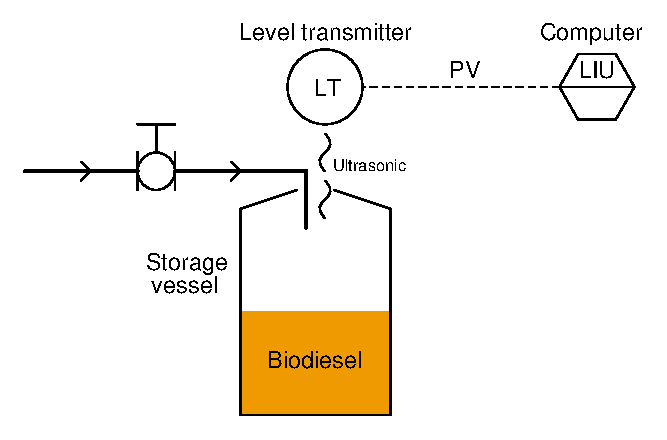
\includegraphics[width=15.5cm]{i01504x02.eps}$$

Væskenivåsignalet fra ultralydnivåtransmitteren (LT) er prosessvariabelen (PV), og det sendes til en datamaskin for indikering og behandling (LIU). Den spesifikke behandlingen i datamaskinen er beregning av gjennomsnittlig strømning mellom samplingsintervaller.

Anta at datamaskinen sampler transmitterens signal én gang per minutt og lagrer målingene i en datafil. Her er et eksempel på innholdet i den filen etter én tankfyllingsbatch, vist i tabellform:

% No blank lines allowed between lines of an \halign structure!
% I use comments (%) instead, so that TeX doesn't choke.

$$\vbox{\offinterlineskip
\halign{\strut
\vrule \quad\hfil # \ \hfil & 
\vrule \quad\hfil # \ \hfil & 
\vrule width2pt \quad\hfil # \ \hfil & 
\vrule \quad\hfil # \ \hfil & 
\vrule width2pt \quad\hfil # \ \hfil & 
\vrule \quad\hfil # \ \hfil \vrule \cr
\noalign{\hrule}
%
% First row
Tid & Volum & Tid & Volum & Tid & Volum \cr
%
(minutter) & (gallons) & (minutter) & (gallons) & (minutter) & (gallons) \cr
%
\noalign{\hrule}
%
% Another row
0 & 17.05 & 10 & 31.12 & 20 & 40.15 \cr
%
\noalign{\hrule}
%
% Another row
1 & 17.05 & 11 & 33.89 & 21 & 42.22 \cr
%
\noalign{\hrule}
%
% Another row
2 & 17.05 & 12 & 36.69 & 22 & 44.60 \cr
%
\noalign{\hrule}
%
% Another row
3 & 17.05 & 13 & 39.40 & 23 & 47.16 \cr
%
\noalign{\hrule}
%
% Another row
4 & 17.05 & 14 & 40.15 & 24 & 50.00 \cr
%
\noalign{\hrule}
%
% Another row
5 & 17.05 & 15 & 40.15 & 25 & 52.85 \cr
%
\noalign{\hrule}
%
% Another row
6 & 20.06 & 16 & 40.15 & 26 & 55.76 \cr
%
\noalign{\hrule}
%
% Another row
7 & 23.01 & 17 & 40.15 & 27 & 58.64 \cr
%
\noalign{\hrule}
%
% Another row
8 & 25.44 & 18 & 40.15 & 28 & 61.53 \cr
%
\noalign{\hrule}
%
% Another row
9 & 28.23 & 19 & 40.15 & 29 & 64.31 \cr
%
\noalign{\hrule}
} % End of \halign 
}$$ % End of \vbox

\filbreak

Plottet over tid får disse dataene følgende form:

$$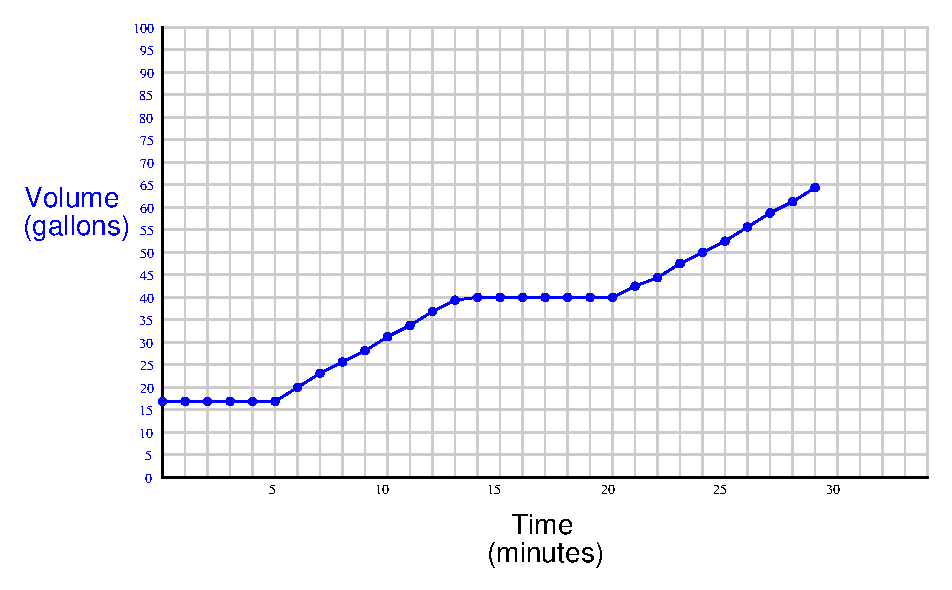
\includegraphics[width=15.5cm]{i01504x01.eps}$$

Bare ved å se på grafen: hva kan du si om {\it strømningsraten} av biodiesel inn i dette karet? Hva kan forklare den ``flate'' delen midt i grafen? Hva representerer de små variasjonene i helning i de andre delene av grafen, når det gjelder strømning inn i karet?

\filbreak

Bruk nå dataene i tabellen til å beregne og plotte biodieselstrømning i gallon per minutt inn i karet:

$$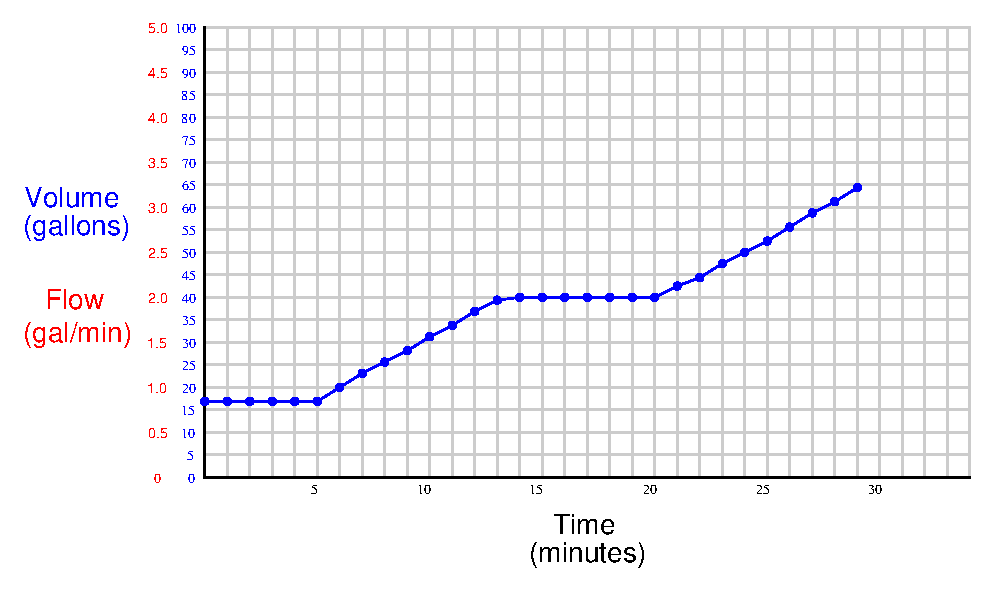
\includegraphics[width=15.5cm]{i01504x03.eps}$$

Hvordan henger de to plottene sammen? Med andre ord: hvordan relaterer {\it formen} på det ene seg geometrisk til {\it formen} på det andre?

\vskip 20pt \vbox{\hrule \hbox{\strut \vrule{} {\bf Forslag til sokratisk diskusjon} \vrule} \hrule}

\begin{itemize}
\item{} Anta at en tekniker ville beregne strømningsraten ved $t =$ 4 minutter ved å ta volumet på dette tidspunktet (17.05 gallon) og dele på tiden (4 minutter). Forklar hvorfor dette gir feil strømverdi, og forklar riktig måte å beregne strømningsraten på ved dette tidspunktet ut fra dataene.
\end{itemize}

\underbar{file i01504}
%(END_QUESTION)





%(BEGIN_ANSWER)

$$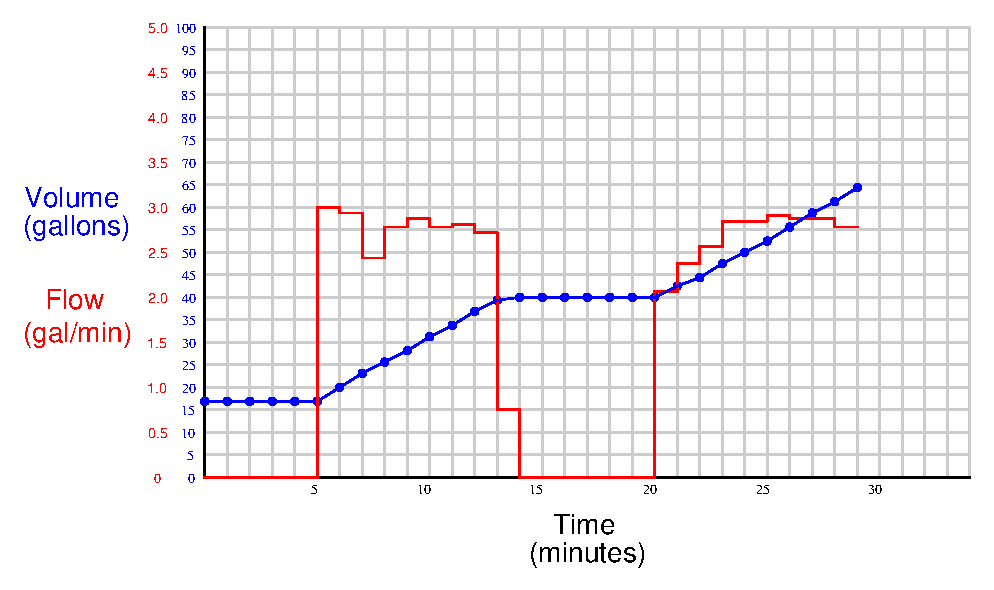
\includegraphics[width=15.5cm]{i01504x04.eps}$$

%(END_ANSWER)





%(BEGIN_NOTES)

Mønsteret bør være tydelig: {\it høyden} på den røde (strømning) grafen ved et gitt tidspunkt speiler {\it helningen} på den blå (volum) grafen. Altså er strømplotet den {\it tidsderiverte} av volumplotet:

$$Q = {dV \over dt}$$

Strengt tatt er det vi beregner her {\it gjennomsnittlig} strømningsrate mellom tidspunkter, representert ved ligningen:

$$Q = {\Delta V \over \Delta t}$$

%INDEX% Mathematics, calculus: derivative (calculating flow rates from measured volumes at specific times)
%INDEX% Process: biodiesel storage tank

%(END_NOTES)

